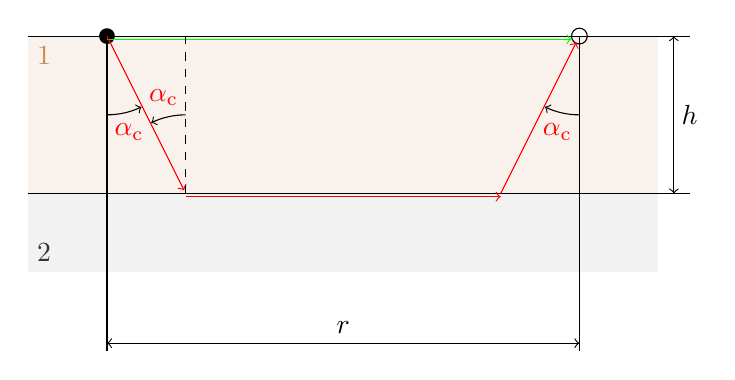
\begin{tikzpicture}
 \fill[brown!10!white] (-2,0) rectangle (6,2);
 \fill[black!5!white] (-2,0) rectangle (6,-1);
 \fill (-1, 2) circle [radius=0.1];
 \draw ( 5, 2) circle [radius=0.1];
 \draw (-1, 2) -- (-1,-2);
 \draw ( 5, 2) -- ( 5,-2);
 \draw[<->] (-1, -1.9) -- ( 5,-1.9);
 \draw (2,-1.7) node {$r$};
 \draw (-2,2 ) -- (6.4,2);
 \draw (-2,0 ) -- (6.4,0);
 \draw[<->] (6.2,0 ) -- (6.2, 2);
 \draw (6.4, 1) node {$h$};
 \draw[->, green] (-1,1.96) -- (4.9, 1.96);
 \draw[->, red] (-1,2) -- (-0.02, 0.04);
 \draw[->, red] (0,-0.04) -- (4,-0.04);
 \draw[->, red] (4, 0) -- ( 4.96, 1.92);
 \draw[dashed] (0,0) -- (0,2);
 \draw[->] ( 0, 1) arc [start angle=90, end angle=116, radius=1];
 \draw[->] (-1, 1) arc [start angle=270, end angle=296, radius=1];
 \draw[red] (103:1.25) node {$\alpha_\mathrm{c}$};
 \draw[red] (-1,2) +(283:1.25) node {$\alpha_\mathrm{c}$};
 \draw[red] ( 5,2) +(257:1.25) node {$\alpha_\mathrm{c}$};
 \draw[->] (5, 1) arc [start angle=270, end angle=244, radius=1];
 \draw[brown!90!white] (-1.8, 1.75) node {$1$};
 \draw[black!80!white] (-1.8,-0.75) node {$2$};
\end{tikzpicture}
